\newpage
\chapter{Projektmanagement}
Anhand der Arbeitsphasen  des Vorgehensmodells werden die folgenden vier Meilensteine definiert. Die Meilensteine markieren jeweils das Ende einer Projektphase und haben einen Fertigstellungstermin. Beim Erreichen eines Meilensteins wird die bisherige Arbeit bewertet und Beschlüsse über den weiteren Projektverlauf gefällt. Insgesamt dienen die Meilensteine dem Projektcontrolling.
\section{Meilensteine}
Es werden die folgenden vier Meilensteine definiert. Die Meilensteine
beinhalten   eine Sammlung von Aufgaben und haben einen
Fertigstellungstermin. Sie markieren das Ende einer Projektphase. Sie
werden für das Projektcontrolling verwendet. 
%\todo{fünf Meilensteine definieren}
	\begin{itemize}
		\item MS1: Theorie und Recherchephase abgeschlossen und zu 80\% dokumentiert, ein Anforderungsdokument wurde erstellt
		\item MS2: Zwischenpräsentation, Vorstellen der ersten vier Antennenkonzepte
		\item MS3: Design und Prototyping, Antennensystem simulieren, produzieren, messen und bewerten
		\item MS4: Engeenieringmodel ist gefertigt und dokumentiert
	\end{itemize}

\section{Projektsitzungen und Gesprächsnotizen}
Die Gesprächsnotizen dienen den Projektverlauf nachvollziehbar zu dokumentieren. Sie werden jeweils nach den Projektsitzungen mit dem Betreuer Prof. Marcel Joss angestellt. Die jeweiligen Arbeitspakete von der vergangenen Woche und der kommenden Woche werden an den Sitzungen besprochen und dokumentiert. Beschlüsse die für den Verlauf der BDA relevant sind werden besprochen und dokumentiert
\section{Vorgehensmodell}
mit Arbeitspaken und Zeitdauer der Arbeits Phasen
\begin{figure}[!ht]
	\begin{center}
		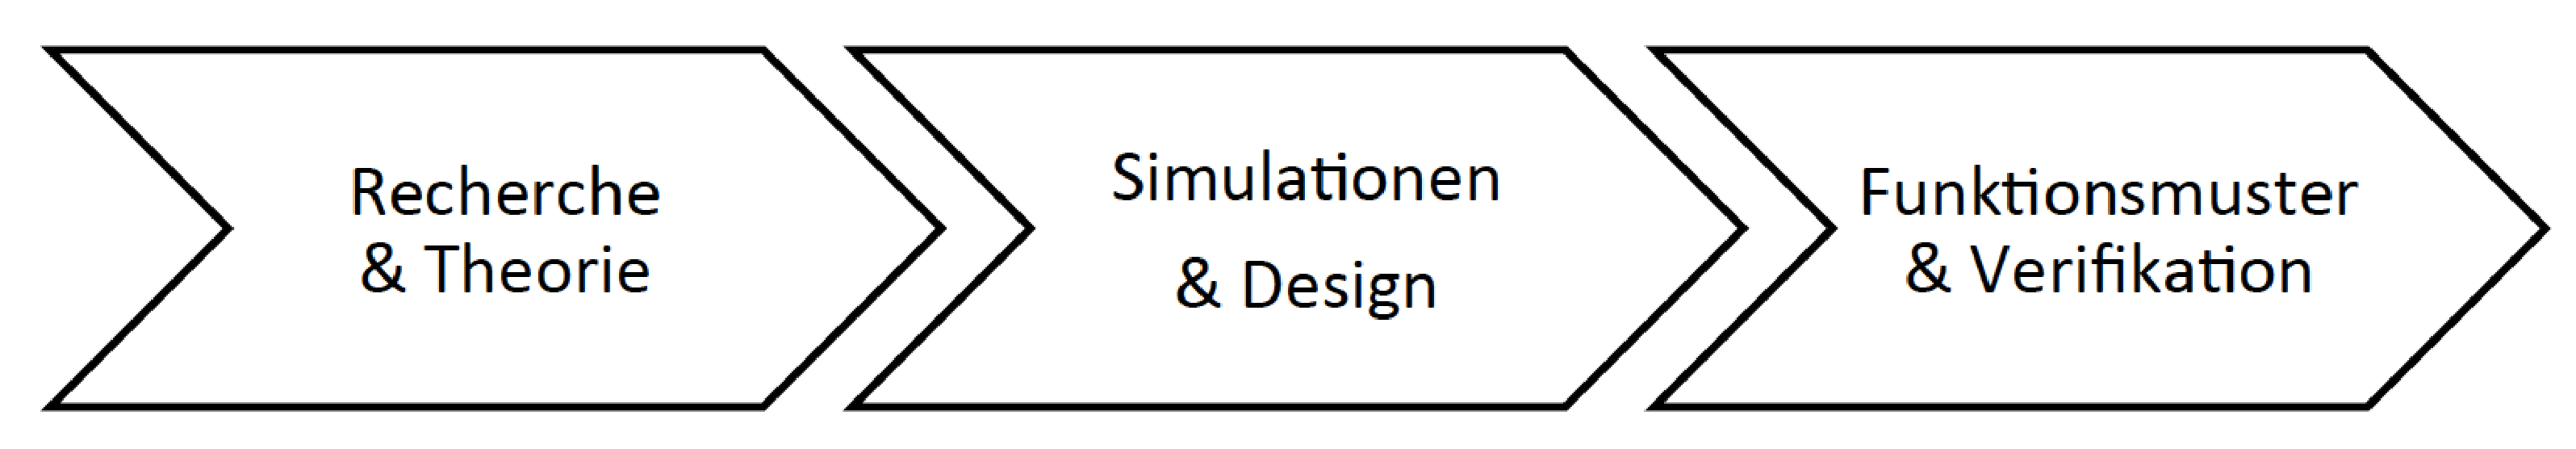
\includegraphics[width=11cm]{content/bilder/Vorgehensmodell.pdf}%
	\end{center}
	\caption{Vorgehensmodell}
	\label{Vorgehensmodell}
\end{figure}
\subsection{Arbeitspakete}
Der Meilenstein 1 schliesst die Recherche und Theorie Phase ab. Die wesentlichen Arbeitspackete sind:
\begin{itemize}
\item Untersuchen, verstehen und beschreiben des Abstrahlverhalten von Elementarstrahlern
\item Die elektromagnetische Feldausbreitung soweit zu verstehen, um diese in einfachen Worten zu beschreiben.
\item Den Zusammenhang von Richtcharakteristik, Wirkungsgrand und Gewinn von verschieden Antennen verstehen und dokumentieren
\item Die Impedanz von Elementarstrahlern untersuchen und beschreien
\end{itemize}
Der Meilenstein 2 beschreibt die Zwischenpräsentation. Dabei wurdend die ersten Resultate aus der Theorie und die ersten Erkenntnisse aus den Simulationen und erste Schlüsse aus den Verglecih idealisierten Theorie und den Simulationen gezogen. 
Konkret wurden die Folgenden Punkte gezeigt:
\begin{itemize}
\item Das Vorgenehnsmodell zeigt die herangehenseise an die BDA
\item Die Feldausbreitung der Elementarstrahler
\item Die Miniaturisierung von Antennen und deren Auswirkung auf Antennenparameter wie: Strahlungswiderstand, Impedanz, Frequenzverschiebung
\item Anahnd des Ersatzschaltbild von einer Hochfrequenzquelle, Leitungen und von einer Antenne wurden Anpassungsschwierigkeiten besprochen
\end{itemize}
Der 3. Meilenstein beinhaltet verschiedenste Arbeitspacke, um einige zu nennen:
\begin{itemize}
\item Impedanz und Resonanzfrequenz  bei Verkürzung von Antennen simulieren
\item die Richtcharakteristik von Loop- und Dipolantennen analysieren und Vor- und Nachteile für die Antennen bewerten
\item Konkrete, umsetzbare Antennendesigns für den einstatz im Fluggerät finden, simulieren und bewerten
\end{itemize}
Der Meilenstein drei endtet mit einem konreten Design welches hergestellt, ausgemessen und bewertet wird.\\
Der 4. Meilenstein beinhaltet das ausmessen und bewerten des Funktionsmusters.
\begin{itemize}
\item Funktionsmuster aus den Designs erstellen
\item Messen der Antennenparameter
\item Vergleich der Simulationen mit den Messwerten
\item Interpretation des Antennendesign und Vergleich mit den Anforderung 
\item Beurteilung des Antennne für den weitern Einsatz in den Fluginstrumenten der Flytec AG. 
\end{itemize}

\subsection{Ressourcenplanung}
Für die Bachelor Dipolom Arbeit wird eine Zeitraum von ca. 360 Stunden eigeplant. Diese Zeit wird auf 15 Wochen an je drei Arbeitstage verteilt. Für die drei Abreitspfasen wurden je etwa dieselebe Zeit, das bedeutet je 5 Wochen eigeplant.\\
Da ausser dem Betreuer Prof. Marcel Joss, dem Industripartner vertreten durch Erich Lerch  und dem Experten xx xx keine weriten Personen in die Arbeit involviert sind, können die Arbetispackete individuell bearbeitet werden und es muss nicht auf dritt Personen rücksicht genommen werden.\\
Die Messeinrichtung wurde während der 3. Arbeitsphase der "Funktionsmuster und Verifikation" nur noch vom Wissenschaftlichen Mitarbeiter und Masterstuden Tobias Pluss verwedent. Es mussten keinerlei Planung stattfinden um keine übeschniedung der Mess-und Analysezeiten zutreffen. 

\subsection{Risikoanalyse}
Wie in der Resourcenplanung erwähnt, war es nicht nötig mit exteren Stellen und dritt Personen für die erreichung der Ziele der Bachelor Dipolm Arbeit zusammen zu arbeiten. Das heisst es besteht keinerlei Risiko mit der Zusammenarbeit mit Exteren stellen.\\
Weiter wurden keine Printantennen in Auftragt gegeben die lange Wartezeiten mitsichgebracht hätten.\\
Die Messeinrichtung stellt auch kein Risiko dar, denn von den meisten Messgeräten sind mehrere oder vergleichbare Exemplare vorhanden.\\
Eine Ausnahem stellt das StarLab dar. Von dieses Antennenmessgerät ist nur eines an der Hochschule für Technik und Architektur. Daher muss auf die einwandfreie Funktion diese vertraut werden. Ist das Gerät nicht funktionstüchtig können keine Abstrahlchakteristiken des Funktionsmuster aufgenommen werden.
